% Created 2021-10-06 Wed 21:21
% Intended LaTeX compiler: pdflatex
\documentclass[11pt]{article}
\usepackage[utf8]{inputenc}
\usepackage[T1]{fontenc}
\usepackage{graphicx}
\usepackage{grffile}
\usepackage{longtable}
\usepackage{wrapfig}
\usepackage{rotating}
\usepackage[normalem]{ulem}
\usepackage{amsmath}
\usepackage{textcomp}
\usepackage{amssymb}
\usepackage{capt-of}
\usepackage{hyperref}
\author{Mridul Gupta (AIZ218322)}
\date{Wednesday 06 October 2021}
\title{COL774 Assignment 2}
\hypersetup{
 pdfauthor={Mridul Gupta (AIZ218322)},
 pdftitle={COL774 Assignment 2},
 pdfkeywords={},
 pdfsubject={},
 pdfcreator={Emacs 27.1 (Org mode 9.3)}, 
 pdflang={English}}
\begin{document}

\maketitle

\section{Q1}
\label{sec:org63bf15d}

\subsection{Q1(a)}
\label{sec:orgfd06dca}
\begin{itemize}
\item Punctutations were removed from the input data, and words containing
numbers like l77t code were also removed.
\item The bag of words model was implemented.
\item Optimal parameters are stored in a pickle file.
\item Train accuracy is \(71.25\%\) while test accuracy is \(66.54\%\).
\item Also, note that I tried to improve the running time to the point I
wrote several different versions of the code, but it just doesn't
get better than 30-40 mins. I hope this counts as \lq\lq
reasonable\rq\rq\ time.
\end{itemize}

\subsection{Q1(b)}
\label{sec:orgeee4adf}
\begin{itemize}
\item Expected random prediction accuracy is \(20\%\). Predicting the
maximum class, the accuracy will be \(66.086\%\).
\item As compared to random prediction, the accuracy gained is \(36.08\%\),
but there is no significant gain compared to maximum prediction.
\end{itemize}

\subsection{Q1(c)}
\label{sec:org31639fc}
\begin{figure}[!htp]
\centering
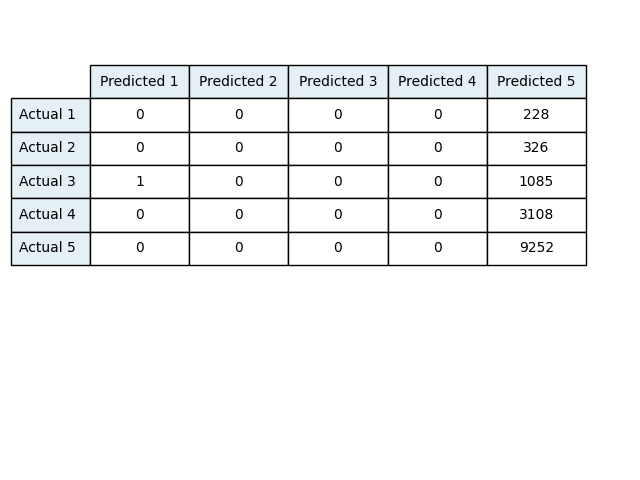
\includegraphics[width=.9\linewidth]{/home/mridul/scai/ml/hw2/src/q1/Confusion_Matrix_1a.png}
\caption{Confusion matrix for Q1(a)}
\end{figure}
\begin{itemize}
\item Class "5" has the highest value of the diagonal entry. This is also
the class with highest number of samples in the training set.
\item It is also seen that classes that have a high prior, pull the
decision towards themselves: most of the false predictions belong to
class "5", then to class "4" and so on. The number of training
samples from each class is listed below.
\item Summing up the column for class "5", we can see 11984 = 85.6\% of
samples are predicted as belonging to class "5". 13.44\% to class
"4", 0.8\% to class "3", 0\% to class "2" and 0.157 to class "1".
\end{itemize}
\begin{align*}
&\text{Category 1:} 2529 =5.05\%\\
&\text{Category 2:} 2638 =5.28\%\\
&\text{Category 3:} 5634 =11.27\%\\
&\text{Category 4:} 13267 =26.53\%\\
&\text{Catgeory 5:} 25932 =51.86\%
\end{align*}

\subsection{Q1(d)}
\label{sec:orgbd97b51}
\begin{figure}[!htp]
\centering
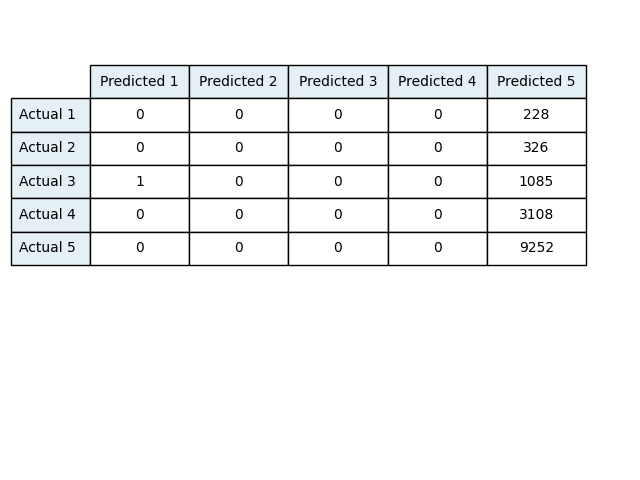
\includegraphics[width=.9\linewidth]{/home/mridul/scai/ml/hw2/src/q1/Confusion_Matrix_1d.png}
\caption{Confusion matrix for Q1(d)}
\end{figure}
\begin{itemize}
\item Accuracy on test set is \(64.77\%\).
\item One would expect the accuracy to improve, but it actually goes down
by 1.77\%.
\end{itemize}

\subsection{Q1(e)}
\label{sec:org1ce0906}
\begin{figure}[!htp]
\centering
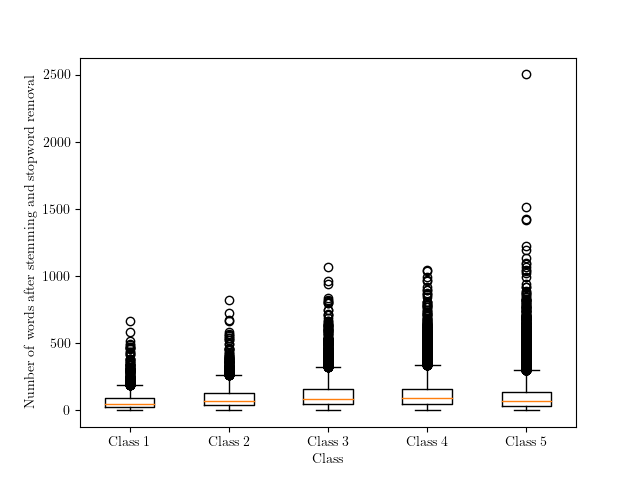
\includegraphics[width=.9\linewidth]{/home/mridul/scai/ml/hw2/src/q1/freq_boxplot.png}
\caption{Frequencies of words}
\end{figure} Features used was
review lengths discretized to four buckets based on boxplot of
classwise lengths plotted. Also, since most of the reviews have
\(<400\) words after removal of stop words but some reviews go on to
contain around 2500 words. We have a lot of data, so in this step I do
not process examples that contain more than 400 words. This can be
seen as a meta feature, to avoid overfitting. I tested with n-gram
extractions, but it was taking a lot of time to train and I didn't
have the resources. So, I ran the n-gram with n=5 on a smaller
dataset, and the accuracy decreased. I didn't pursue it further. The
accuracy is no still around \(65\%\) but there is some speed gain as
we are not processing long reviews.

\subsection{Q1(f)}
\label{sec:org7318bc7}
The class-wise F1-scores and macro F1-score are:
\par
\begin{center}
\begin{tabular}{cc}
Class 1 & 26.95\%\\
Class 2 & 4.70\%\\
Class 3 & 18.77\%\\
Class 4 & 34.54\%\\
Class 5 & 80.36\%\\
Macro F1 & 33.07\%
\end{tabular}
\end{center}
\par
The macro F1-score and the per class F1-scores is more suited in this
kind of dataset as the dataset is imabalanced, and this metric gives
insights into the performance per class. An extreme case might be of
cancer cell detection from images, where we might have very few
examples of the positive class. But it will be crucial to classify
them correctly so that a patient gets correct treatment on time and a
healthy person doesn't has to go through the treatment.


\subsection{Q1(g)}
\label{sec:orge6ae106}

I tried training a Naive Bayes model when summaries were just added as part of
the review. Since Naive Bayes is a stable model, and the summaries are small and
very likely to be correlated to the review, the results didn't change much.\par
Next, I tried implementing a separate Naive Bayes model using just the summaries
and calculated actual probabilities from the unnormalized log probabilities of
the two models, and just chose the prediction of the one which was confident.
The accuracy is still around 65\%. But all this does is make the prediction go
more towards max prediction as seen from confusion matrix.
\begin{figure}
	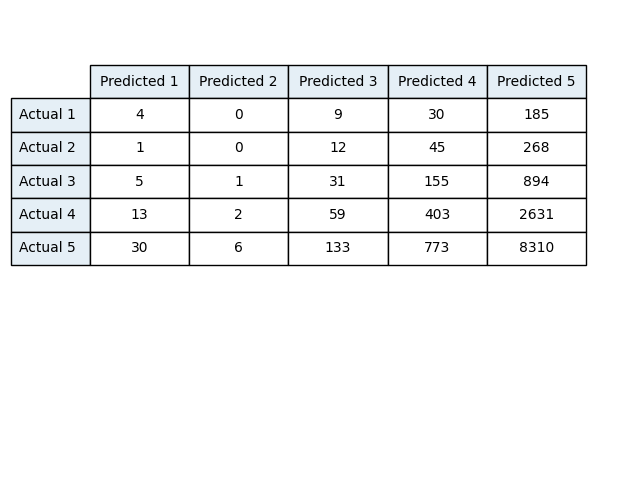
\includegraphics[width=0.9\textwidth]{/home/mridul/scai/ml/hw2/src/q1/Conf1g.png}
	\caption{Confusion matrix for Q1(g)}
\end{figure}
If I had time, I'd have implemented a Naive
Bayes model with some random words dropped out to create a third model and used
these in ensemble.
\section{Q2}
\label{sec:orgfc0fbfa}

\subsection{Q2(a)}
\label{sec:org1b1d25b}
\subsubsection{i)}
\label{sec:orgb1d3619}
Accuracy on training data is \(99.28\%\). Accuracy on test data is
\(97.26\%\). There are 309 support vectors in this case.

\subsubsection{ii)}
\label{sec:org1f15d28}
Accuracy on training data is \(100\%\), while on test data is
\(99.02\%\). There are 1856 support vectors in this case. The accuracy
improves as compared to when using linear kernel, but so does the
computation time. And in this particular case, the gain in accuracy is
not enough to justify the loss in computation time.

\subsubsection{iii)}
\label{sec:orgeed620b}
\begin{itemize}
\item linear: nSV = 297. Test set accuracy is \(97.01\%\). Training and
testing times are 10\(\times\) faster than my cvxopt implementation.
\item gaussian: nSV = 1823. Test set accuracy is \(99.26\%\). Training and
testing times are 20\(\times\) faster than my cvxopt implmentation.
\item As noted \href{https://stackoverflow.com/a/5333279}{here}, it is not possible to extract weights and bias from
the svm model created by libsvm in python. I did not compare them.
\end{itemize}

\subsection{Q2(b)}
\label{sec:org26d97bb}
\subsubsection{i)}
\label{sec:org2c05647}
Test set accuracy is \(96.84\%\). The testing process is very slow
though, takes around 15 minutes on the test set of \(10^4\)
samples. Training time is around 70 minutes.

\subsubsection{ii)}
\label{sec:orgf28d3ee}
Test set accuracy is \(97.23\%\). The accuracy is not significantly
different from the cvxopt implementation. Without any information
about SVM performance on the given dataset other than the cvxopt
implementation, the expected accuracy is \(96.84\%\). According to
Markov inequality then, \(\displaystyle P[\text{acc}\ge 97.23]\le
\frac{96.84}{97.23}=0.9959\). That is to say, this is not such a rare event.

\par The testing time is 1.5 minutes. Training time is around 3
minutes. Around 25 times faster.

\subsubsection{iii)}
\label{sec:org9f2c6a0}
\begin{figure}[!htp]
\centering
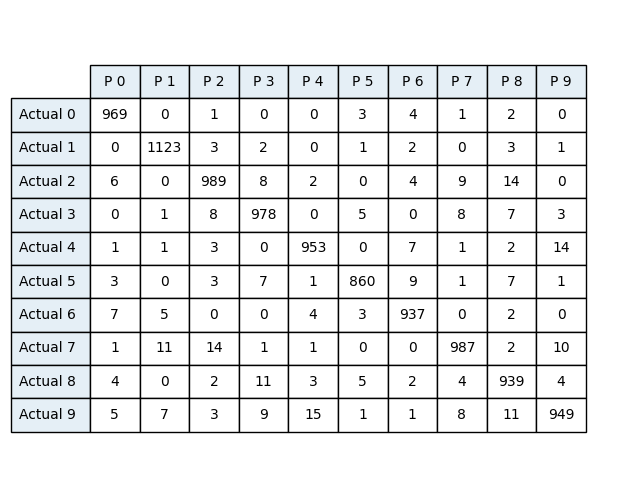
\includegraphics[width=.9\linewidth]{/home/mridul/scai/ml/hw2/src/q2/cvxopt_multi.png}
\caption{Confusion matrix for o-v-o SVM using CVXOPT}
\end{figure}
\begin{figure}[!htp]
\centering
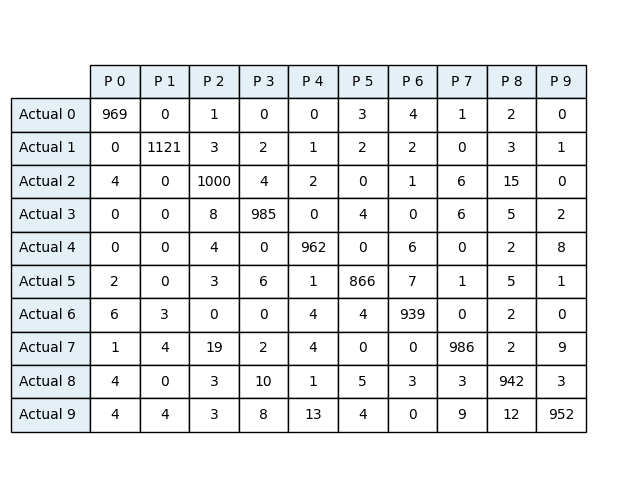
\includegraphics[width=.9\linewidth]{/home/mridul/scai/ml/hw2/src/q2/libsvm_multi.png}
\caption{Confusion matrix for o-v-o SVM using LIBSVM}
\end{figure}
\begin{figure}[!htp]
\centering
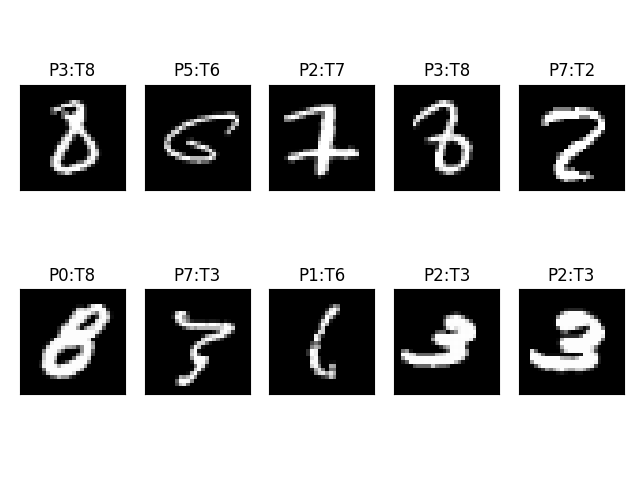
\includegraphics[width=.9\linewidth]{/home/mridul/scai/ml/hw2/src/q2/cvxopt.png}
	\caption{Misclassified images by SVM using CVXOPT\label{mis}}
\end{figure}
\begin{figure}[!htp]
\centering
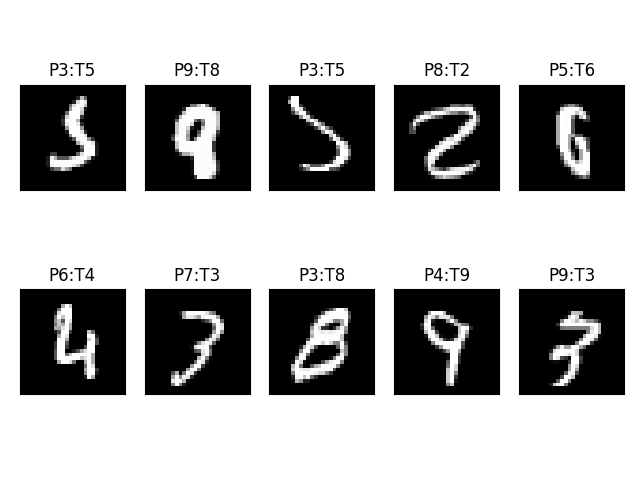
\includegraphics[width=.9\linewidth]{/home/mridul/scai/ml/hw2/src/q2/libsvm.png}
	\caption{Misclassified imaged by SVM using LIBSVM\label{mis1}}
\end{figure}
The images misclassified by the models shown in figures~\ref{mis}-\ref{mis1} are confusing to my eyes as
well. Some of them are written in poor handwriting or incomplete, and
trying to complete them one can go two ways, the predicted and the
true label.
\par
For cvxopt\\
0 is usually confused as 6
1 is confused as 2, 3, 4, 6, 3 and 9\\
2 mostly with 8, 7 and 3.\\
3 as 2, 7 and 8.\\
4 as 9.\\
5 as 6, 3 and 8.\\
6 as 0.\\
7 as 2, 1 and 9.\\
8 as 3\\
9 as 4 and 8.\\
Similar trends hold for libsvm implementation as well.

\subsubsection{iv)}
\label{sec:orge40a797}
Value of C that gives best accuracy for 5-fold cross-validation
is 5. This is also the value of C that gives the best accuracy for
test set.\par
The graph in figure \ref{kfold} shows that even though there is some variation, the 5-fold
cross-validation accuracies and the test set follow each other closely.
\begin{figure}[!htp]
\centering
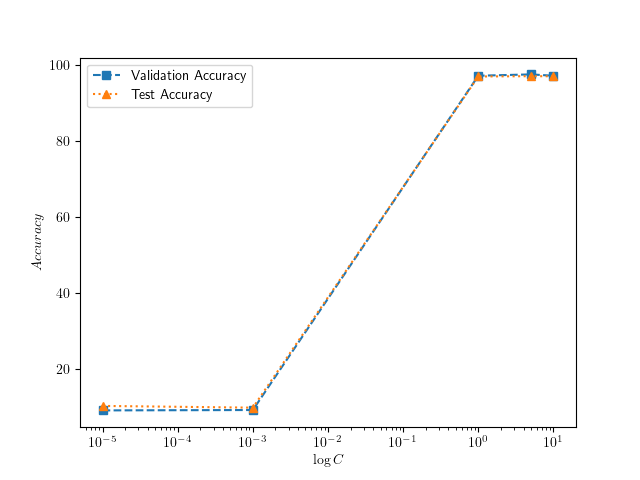
\includegraphics[width=.9\linewidth]{/home/mridul/scai/ml/hw2/src/q2/kfold_cross_validation.png}
	\caption{Cross-validation versus test set accuracies\label{kfold}}
\end{figure}
\end{document}
